\chapter{Introduction}

\section{Introductory material}

\subsection{JNDD introduction}
Reading is a complex cognitive act. To read, individuals must precisely control visual attention, map symbols to phonological representations, extract meaning from words, update mental representations of the text, inhibit unimportant associations, and make appropriate inferences. Consequently, while the most explicit aim of reading instruction and intervention is to build fast and efficient orthographic-phonological mapping, reading difficulty can arise from many sources \cite{Pennington2009, vanderLely2010}. To further complicate matters, reading disability is often comorbid with other learning and developmental disorders, such as specific language impairment and attention deficit / hyperactivity disorder \cite{Pennington2006, Margari2013}.

In the past two decades, neuroimaging research has provided valuable insights into the neural mechanisms of typical and atypical reading. Researchers have found that reading co-opts the brain's visual system to introduce a new input pathway into existing language comprehension circuitry \cite{Jobard2007}. As text complexity increases, a larger demand is made on attentional systems, and activation becomes more bilateral and widespread \cite{Xu2005}.  Meta-analyses show that individuals with reading difficulty typically exhibit underactivation in areas responsible for recognizing symbol units, parsing acoustic sounds into phonological units, and binding letters to sounds \cite{Maisog2008, Richlan2009, Paulesu2014}. However, many questions remain regarding the root causes of dyslexia, how to best identify children at risk and the reasons for its high comorbidity with other developmental disorders. 

Connectivity-based neuroimaging methods provide an alternative framework to examine reading difficulties. Whereas traditional  approaches focus on identifying focal regions of deficit, many learning and psychiatric disorders are characterized, in part, by how brain networks behave and interact. In particular, \textit{connectomics} analyses have shown that the brain exhibits a network configuration which allows for high transferability of information at minimal cost, i.e. a “small-world” network architecture \cite{Bullmore2012}. Two attributes of brain organization have been of special interest: the presence of densely intra-connected \textit{modules}, often called resting-state networks (RSNs) \cite{Sporns2016}; and the existence of a core group of \textit{hub areas} that play an outsize role in conveying information between RSNs \cite{VandenHeuvel2011}. 

Since reading requires rapid interaction and manipulation of disparate cognitive processes, the network framework is an appealing avenue of investigation in reading disorders. Previous research has suggested that the areas responsible for reading do not form a single network, but are instead distributed across multiple RSNs \cite{Vogel2013}. There is evidence that the constitution of these RSNs (e.g. the default mode network) could be predictive of disorders, including attention deficits \cite{Uddin2008}. Furthermore, damage to hub areas can cause devastating behavioral effects \cite{Warren2014} and may be degenerated in psychiatric and developmental disorders such as schizophrenia, Alzheimer's disease and ADHD \cite{Stam2014}. Graph theory measures of connectedness within and between RSNs may consequently be related to differences in reading skill. However, while a small number of papers indicate that they may be affected in dyslexia \cite{Qi2016, Finn2014}, its application in the reading domain has been relatively sparse, with few emergent themes thus far \cite{Cao2016}. This is surpising because connectomics data can be procured without using cognitive tasks (which represent a confounding variable) and because they provide a common neurobiological framework for understanding cognitive disorders.


\subsection{VRN introduction}

Comprehending text is a necessary skill in modern civilization, but a large percentage of people struggle with it. In Nashville, for example, 1 in 8 adults is illiterate. Often reading difficulty is caused by poor word recognition, or trouble mapping word sounds (phonology) onto symbols (orthography). However, even when individuals are able to recognize words, they may struggle with comprehending the text's primary message. While several skills important for fluent comprehension have been identified, including phonological awareness, vocabulary and attention, diagnosing and assisting poor comprehenders remains difficult. This has motivated researchers to investigate the biological basis for reading, which may provide insight into whether fluent comprehension is more than simply the sum of its parts. 

Much of our current understanding of the brain basis for language stems from a scientific tradition of localization. Nineteenth century phrenologists culled insights about personality and aptitudes from skull structure; twentieth-century neurologists used brain damage to infer cortical specialization. More recently, scientists have used functional magnetic resonance imaging (fMRI) to map brain activity during cognition, from the simple (finger tapping) to the sophisticated (language comprehension). In the case of reading, neuroscientists have converged on a set of regions constituting a basic reading network in the left hemisphere, including occipito-temporal for word recognition, temporo-parietal for semantic processing and inferior frontal areas for articulation and encoding  \cite{Price2012}. However, in the case of comprehension, it is clear that brain areas do not act on their own but in concert. Damage to the white matter tracts connecting them can have as devastating consequences as damage to the cortical areas. Indeed, even damage to areas that are not considered primary to language can have a debilitating effect: right hemisphere lesions can affect how well an individual can understand the metaphorical meaning or emotional salience of text \cite{Ferstl2008, Vigneau2011}.

The appropriate level of investigation for understanding reading comprehension, rather than the cell, circuit or gyrus, may thus be the \textit{network} of brain areas. In this review, we discuss network theories of reading development and then explore how one approach to network analysis -- graph theory --  has been used to relate network properties to behavioral indices of cognition. Finally, we discuss the future of these approaches and the potential benefit they may confer. 


\subsection{VRN section on specialization}

In the United States, children are taught to decode words between the ages of four and nine. This is a time of major developmental changes in the brain, including synaptic pruning and myelination \cite{Wandell2013}. Reading development thus occurs during a period of both active intrinsic development and structured extrinsic instruction. The brain areas responsible for fast and efficient word decoding may become specialized through a process of \textit{interactive specialization}, in which intrinsic developmental processes and experience collaborate to form the mature, skilled reading system \cite{Johnson2011, Klingberg2014}. The theory is built on the Hebbian maxim that "neurons that fire together, wire together", with the brain being considerably more plastic during this developmental period than it is later in life \cite{Hebb1949}.

n important step in building reading skill is learning to recognize words by sight (e.g. to be able to quickly and automatically associate the sound /kat/ with the letters \textit{C-A-T}). This is mediated through a portion of the fusiform gyrus: neural activity appears to become increasingly specific to words as individuals become better at recognizing words \cite{Mccandliss2003, Schlaggar2007}. Consistent co-activation between early processing areas in the visual cortex and the fusiform gyrus may create long-lasting correlations between neuronal activity in the two areas. Failure to develop this sensitivity to word stimuli may be one of the causes of poor reading \cite{He2013}.  

This process of interactive specialization may cause lasting changes to connectivity even when subjects are not reading. Evidence for this comes from resting-state fMRI, which does not require individuals to complete tasks but instead uses spontaneous neural activity from the fMRI signal to construct networks. Koyama et al. found that many reading-related nodes had overlapping connectivity with the left inferior frontal gyrus and left middle temporal gyrus, both nodes that are important for skilled language use \cite{Koyama2010}. A follow-up study comparing IQ-matched children and adults found similar patterns: better readers in both groups showed increased connectivity between the inferior frontal gyrus and the middle and superior temporal gyri, as well as between the precentral gyrus and motor areas \cite{Koyama2011}. In adults, positive correlations were found between reading ability and connectivity between the visual word form area and phonological processing areas; in children, however, this correlation was weaker and negative, suggesting that the visual word form area becomes more integrated with experience as well as skill. Reading intervention also exerts an effect on connectivity patterns. Dyslexic adolescents who received reading remediation had higher correlations between the visual word form area and the right middle occipital gyrus than did control participants \cite{Koyama2013}. This connectivity also correlated with spelling and single-word reading scores.

However, word recognition skill is insufficient to explain individual differences in comprehension \cite{Gough1986, Hoover1990}. That is, comprehension requires more areas of the brain than do those of more basic reading skills. Xu et al. reported that in single-word reading tasks, neural activity is largely confined to areas near the visual system in fusiform regions, whereas in sentence and passage comprehension, readers utilize a broader array of brain regions \cite{Xu2005}. In an fMRI scanner, participants read a stream of words, followed by a stream of sentences and finally a full narrative. Across all three levels, there was activation in perisylvian language areas. Sentence processing correlated with increased activity in the bilateral temporal poles. However, when the same sentence stimuli were presented within the context of a narrative, the authors found large activations across both hemispheres, including the precuneus, medial prefrontal and dorsal TP and occipital cortex. 

Other reports corroborate these larger activations: Cutting et al. used a sentence comprehension task which elicited bilateral temporal lobe activation (left \textgreater right) and greater occipital lobe signal, as would be expected from increased language and visual load. Thus, sentence comprehension relies on a core set of extended language regions above that required for words.  \cite{Cutting2006a}. Consistent with theory, as readers become more skilled, patterns become more focused and sharply defined; in contrast, those who continue to struggle with reading (i.e. dyslexia) continue to show a more diffuse pattern of activity \cite{Rimrodt2009}. 

To investigate interactive specialization in comprehension and other multifaceted behaviors, looking at single connections between areas of the brain may not be sufficient. Instead, the properties of the larger system of brain areas must be accounted for. 

\section{Examples of networks and network methods}

\subsection{Resting-State Networks}
In 1995, Biswal et al. discovered that portions of motor cortex that were active during tasks were also correlated with each other areas at rest, suggesting that there was an intrinsic connectivity between these areas \cite{Biswal1995}. However, in the excitement of the early years of fMRI, these non-task-related findings were of little interest. In 2003, Greicius et al. found that the "default mode network", a set of brain areas that was commonly seen anti-correlated during tasks, was found to be active at rest \cite{Greicius2003}. Since then, scientists have been actively identifying and characterizing intrinsic resting-state networks (RSNs) that can be reliably found in individuals at rest. A number of RSNs have been identified which may underlie cognitive function, including language \cite{Cordes2000, Hampson2002}, visual perception \cite{Cordes2000, Simmons2012}, motor functioning \cite{Biswal1995} and executive control \cite{Seeley2007, Simmons2012}. Although there can be significant variability between and even within scans \cite{Honey2009}, these functional connectivity findings are robust and have been repeatedly found in large scale datasets.

\begin{figure}[t]
    \centering
    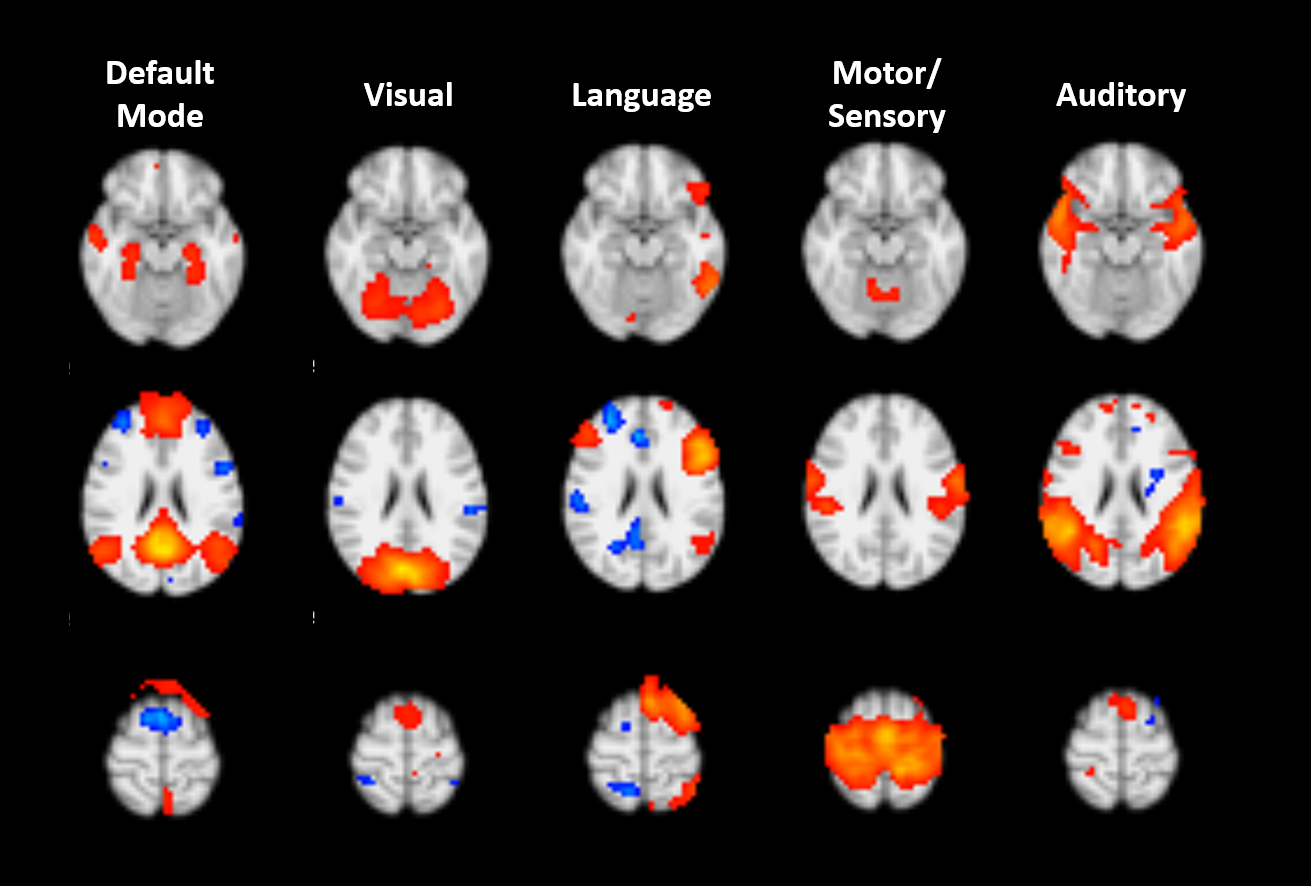
\includegraphics[width=12cm]{Ch1_ICA}
    \caption[Examples of resting-state networks.]{Examples of resting-state networks derived from 16 adult subjects at rest. fMRI data were decomposed into 21 independent components and thresholded at p \textgreater 0.7.} 
\end{figure}

Beyond simply identifying these networks, scientists have used graph theory to analyze how the brain areas that make up these networks act in terms of the entire system of brain networks (sometimes called the connectome). In graph theory, each brain area is a single "node" in the larger brain network and temporal correlations with other nodes are "edges". In RS-fMRI, similar cortical areas (e.g. Brodmann areas) are typically assigned to to be nodes. In some cases, the entire brain is input into the analysis, whereas others use a more targeted, seed-based approach \cite{Vogel2010}.  Edges are often weighted, meaning areas that are more highly correlated carry a greater connectivity value. Next, an algorithm is applied to the matrix of correlations to distinguish sets of nodes that are more highly connected to each other than to other areas of the brain. Finally, first- and second-level properties of the networks, are derived.

The decision of which regions to include as nodes is critical. Typically, one of several approaches has been used to identify nodes: anatomical parcellations based on an atlas \cite{Supekar2008, Liu2008, Lynall2010}; individual voxels \cite{Fair2007}; functional ROIs from either a priori hypotheses or task-based activation \cite{VandenHeuvel2010}; or an algorithm that parcellates the brain independent of function or anatomy \cite{Goni2014}.  Differences in these methods can affect the RSNs identified. At high resolutions (e.g. voxel-level correlations), there is a greater chance of spurious correlations causing noise in the data; at lower resolutions, the timeseries for a region may blend multiple functional regions, creating a composite that does not truly reflect any of the underlying areas. 

Graph theory provides several metrics for consideration, of which we discuss three: \textit{node degree} is the number of connections a single node has \cite{Sporns2013}. Nodes with higher degrees are thought to communicate with a greater number of nodes than others; networks with a higher average degree are thought to be more densely connected. \textit{Path length} is the minimum number of nodes that must be passed to connect one node to any other. A completely random network will have a relatively low path length; a completely regular one will have a high path length. Finally, the \textit{participation coefficient} is the degree to which a node participates in networks other than its primary one. These properties have been used to find a number of interesting things about the brain. 

Developmentally, RSNs exhibit increasing functional correlation across the lifespan \cite{Kesler2013, Uddin2010}. Properties of these RSNs, including density of connections, along with their locations and changes with development is of primary interest  \cite{Cole2014, Dosenbach2007, Fair2009}. RSNs in children are more greatly constrained by proximity than in adults but are functionally organized: visual system regions, for example, form their own community, as do auditory regions and executive control regions \cite{Seeley2007}. Several studies report that the brain takes on a modular structure, consisting of many densely intra-connected networks \cite{Bullmore2009, Fair2009, Supekar2009, Dosenbach2007}. These modules are connected to each other by a smaller number of regions, dubbed "rich clubs" or "hubs", that may facilitate the passage of information from one module to another \cite{Power2013, Bullmore2012}. 

\begin{figure}[t]
    \centering
    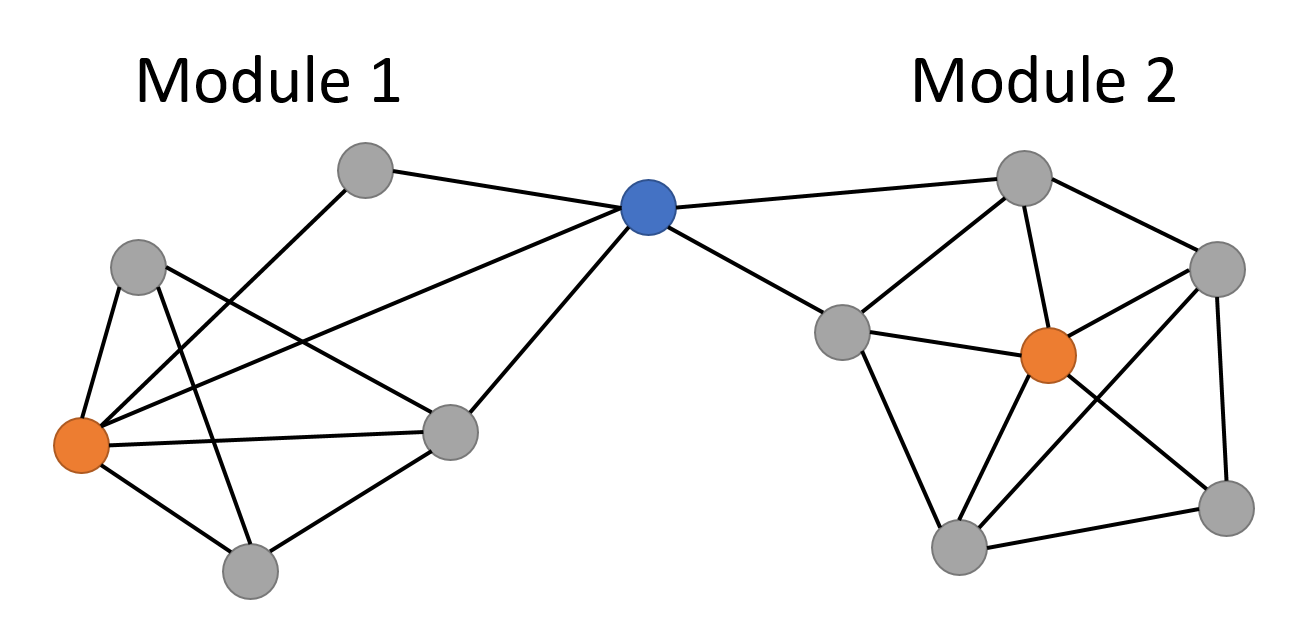
\includegraphics[width=14cm]{Ch1_GraphSchema.png}
    \caption[Schematic for a network with two modules.]{Schematic for a network with two modules. The blue node is a hub region critical for connecting modules 1 and 2. The orange nodes have the highest degree of all nodes.}
\end{figure}

\subsection{VRN: General applications of graph theory}

These findings have informed our understanding of the brain's large-scale organization. Rather than having a set of tracts that connect all regions, these findings suggest the brain is organized complexly but efficiently in a "small-world" architecture. This has emphasis on the importance of certain regions to fulfilling cognitive functions: in one study with lesioned patients, Petersen et al. predicted how severe a lesion would be based on its proximity to these hub regions \cite{Warren2014}. They found that lesions on areas that were not densely connected showed less extended impairments than regions which were highly inter-connected in RS-fMRI. Other psychiatric disorders have found disruptions in network properties. Lord et al. found that while whole-brain metrics of modularity were similar across individuals with depression and , RSNs "reorganized" in individuals with depression \cite{Lord2012}. Thus network properties may be important for explaining individual differences in neuropsychiatric disorders or cognitive skill, such as comprehension. 

Relatively few studies have been done relating network methods to reading ability. Despite the changes in connectivity between areas, reading-related regions such as the fusiform gyrus, angular gyrus and inferior frontal gyrus, do not create one distinct RSN, but are members of separate, more primary RSNs \cite{Vogel2013}. Finn et al. compared graph theory metrics of dyslexic and non-impaired readers using graph metrics \cite{Finn2014}. Dyslexic readers showed divergent activity in visual association and prefrontal attention areas as well as increased right-hemisphere connectivity. Differences were persistent across both adult and children readers, suggesting that network metrics are relevant for reading. Another study investigating how graph theory metrics changed in response to sentence-level processing showed that network properties were relatively stable \cite{Ye2012}. Participants were asked to silently read a sentence that had either a semantically congruent or incongruent ending. Furthermore, metrics showed that subcortical processing (basal ganglia to supplementary motor area) was stronger in response to incongruent versus congruent endings. 

According to the view of interactive specialization, an integrative ability like reading comprehension would be more highly connected. The multi-RSN robustness, or the how well-maintained the network is after deletion of a node, will measure how strongly inter-connected the RSNs of interest are to each other \cite{Bullmore2009}. An important consequence of these hypotheses is that, if there is a biological substrate underlying RC, we may have another window into predicting how well a child will continue to develop as a reader, especially during the periods of rapid development in primary school.

One promising area of application is that of prediction. Machine learning techniques such as multivariate pattern analysis have been used to classify individuals with developmental and neuropsychiatric disorders before, including individuals with dyslexia \cite{Ecker2010, Hoeft2011, Wee2014, Hoeft2007, Ingalhalikar2014}, autism and depression \cite{Lord2012}.  These techniques can incorporate multiple sources of information, such as network properties, to build the optimal model for predicting whether a dataset belongs in one group relative to another \cite{Pereira2009}. This has been done with anatomical and functional data \cite{Hoeft2007, Hoeft2007b}. Network properties may be even more likely to contain information about an individual's likelihood of succeeding in school than other metrics.

However, the neurobiological basis for these RSN properties is still under investigation. While these connections do appear to be plastic and mediated by experience, they are not necessarily caused by new synapses. Several studies using diffusion-weighted MRI (DW-MRI) suggest that functional connectivity represents more than simply direct synaptic connections. DW-MRI uses water movement to model the white matter tracts within the brain. At high resolutions, it provides a coarse approximation of the human connectome -- the total connections in the human brain \cite{Sporns2005}. Honey et al. investigated whether functional connectivity can be predicted from structural connectivity \cite{Honey2009}. Five subjects underwent DW-MRI and RS-fMRI scans, and brains were parcellated at both a high resolution (998 cortical regions) and low resolution (66 cortical regions). They found that, while structurally connected areas are typically functionally connected as well, the inverse is not true. Areas that were closer together were also more highly functionally connected, possibly due to structural cortico-cortical projections. 

More work, including longitudinal studies, certainly needs to be done to understand the complex processes. One of the outstanding questions in the field, though, is what (and even whether) these properties have a neural or psychological basis. While it is likely that RSNs reflect a long history of co-activation between brain areas \cite{Cohen2008, Fair2008}, it is less clear what individual differences in a specific metric might mean.


\subsection{Distribution of resting-state networks across reading areas}
Reading-related regions were selected on the basis of the Neurosynth meta-analytical database \cite{Yarkoni2011}, comprising 11,406 studies as of October 31, 2017. NeuroSynth aggregates brain activation data from thousands of studies to return activation likelihood maps based on search terms. The database was queried for "reading", yielding 427 studies. NeuroSynth provides two meta-analysic activation maps, one using forward-inference and the other using reverse-inference. The forward-inference map creates a map of brain areas associated with reading-related papers; the reverse-inference map returns the set of brain areas most likely to be active only in reading-related papers. The reverse-inference map thus de-weights domain-general functional areas and is more representative of reading-specific areas than the forward-inference map. Because domain-general processes are fundamental to skilled reading (especially comprehension), our primary interest was in the forward-inference map, but both maps were examined. 

The 7-network cortical parcellation from Yeo and colleagues (2011) was used to represent canonical RSNs \cite{Yeo2011}. On the basis of resting-state fMRI data from 1000 subjects, this atlas identifies the following RSNs: visual, somatomotor/auditory, limbic, ventral attention, dorsal attention, default mode, and fronto-parietal. The "Liberally Masked" volumetric data was downloaded in MNI152 space and co-registered to the NeuroSynth data. For each inference map, the percentage of activation falling into each RSN (cm\textsuperscript{3}) was calculated to provide a distribution across each RSN.

A comparison of the NeuroSynth "reading" activations to the 7-network parcellation from Yeo and colleagues shows that reading is widely distributed across resting-state networks (Fig. 1). In the forward-inference map, the visual and somatomotor-auditory RSNs consituted about one quarter of the NeuroSynth activations (17.5 and 8.2 percent, respectively), while attention networks combined to make up 37 percent. The fronto-parietal (19.3 percent) and default mode (17.8 percent) networks were were also highly represented. The limbic network was the only RSN which did not meaningfully overlap with the reading network. Compared to the baseline distribution of the Yeo parcellation, the visual, dorsal attention, ventral attention and fronto-parietal networks consituted a larger portion of the activation; the limbic, somatomotor and default mode had smaller shares (Table 2). 

The NeuroSynth reverse-inference map was smaller than the forward-inference map by 28.7 percent and was restricted to areas more specific to reading. In particular, there was a higher involvement of the visual (+3.9 percent) and default mode network (+11.8 percent) compared to the forward-inference map. On the other hand, networks supporting domain-general functions (dorsal attention, ventral attention, fronto-parietal) were relatively less present (-3.4, -6.7 and -6.0 percent, respectively). Representation of the somatomotor-auditory and limbic network involvement was mostly unchanged.

\begin{figure}
\centering
\includegraphics[width=5in]{Ch1_YeoReading.png}
    \caption[Reading areas are distributed across many resting-state networks.]{Reading areas are distributed across many resting-state networks. On the left is the volumetric breakdown of the "reading" network, pulled from a NeuroSynth automated meta-analysis (forward-inference: $p < 0.01$, FDR-corrected) \cite{Yarkoni2011}, according to the 7-network cortical parcellation from Yeo and colleagues \cite{Yeo2011}. On the right is a surface plot of the same data. Reading areas are well-distributed across different networks and load highly onto attention and executive networks. Several important reading areas, including the inferior frontal gyrus and temporo-parietal junction, sit at points where multiple networks converge, i.e. likely hub areas.}
    \label{fig:texlogo}
\end{figure}



\subsection{Graph theory analyses}


\subsection{Mapping dyslexia abnormalities onto hub areas}
Two decades of neuroimaging research have allowed a relative consensus to form as to which brain regions are commonly dysfunctional in dyslexia. To determine whether there was any pattern related to network architecture in these areas, we gathered all clusters from three meta-analyses comparing fMRI activation for individuals with dyslexia to typical readers \cite{Maisog2008, Richlan2009, Paulesu2014}. All areas that showed atypical activation in dyslexia (either greater or less activity) were included. When a cluster was large, all reported local maxima were included. 

To get measures of hubness across the brain, we used data from a connectomics study by Power and colleagues (2013) \cite{Power2013}. That study reports the \textit{participation coefficient} for each of the 264 nodes previously described. The participation coefficient reflects the diversity of a node's connectivity to different RSNs, where a higher value indicates that the node is correlated with many different RSNs. Activations from the dyslexia meta-analyses were then mapped to the geometrically closest node from this dataset, resulting in a small set of dyslexia-related nodes and a larger, unaffected set.

The distribution of participation coefficients across the 264 nodes was non-normal, with a large group of areas having low participation coefficients (i.e. affiliated with few RSNs) and a smaller hub-like group. Therefore, a Wilcoxon rank-sum test was performed on the participation coefficients for the two groups, which tests for the equivalence of two distributions in a non-parametric fashion.

Across the three meta-analyses, 32 of the 264 nodes showed abnormal functioning in dyslexia. Figure 3 shows the node-by-node distribution of participation coefficients for the entire set. The median participation coefficient for unaffected nodes was 1.47; for dyslexia-related nodes it was 3.28. A Wilcoxon rank-sum test between the dyslexia and unaffected nodes showed that dyslexia affects brain areas with higher participation coefficients than would otherwise be expected ($U = 4946.0$, $p$ \textless $0.001$). 


\begin{figure}[h!]
\centering
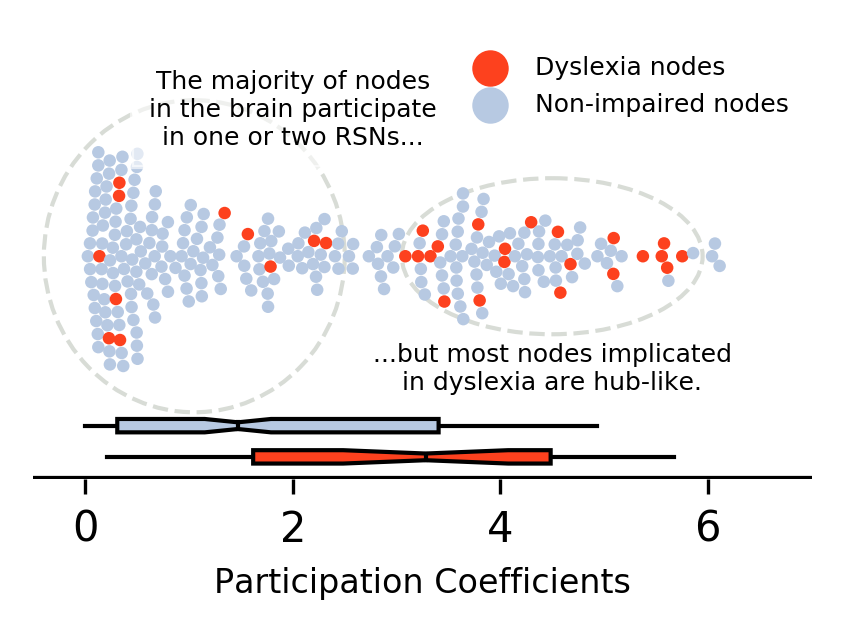
\includegraphics[width=5in]{Ch1_DyslexiaHubs.png}
    \caption[Dyslexia disproportionately impacts hub areas.]{Dyslexia disproportionately impacts hub areas. Among the brain areas examined in Power and colleagues (2013), nodes implicated in dyslexia have higher participation coefficients (32 nodes) compared to the rest of the brain (232 nodes).}
\label{fig:texlogo}
\end{figure}